\chapter{Đọc thêm 2: Xử lý Dữ liệu Tần suất Siêu cao (Brownlees \& Gallo)}
\label{ch:M3L3DT2}

% Nguồn: Brownlees, C. T., & Gallo, G. M. ``Financial Econometric Analysis at Ultra-High Frequency: Data Handling Concerns.'' Computational Statistics & Data Analysis, 51(4), 2006, pp. 2232-2245.
% Phần cần đọc: Sections 3.1-3.2
% Nội dung bắt buộc đọc: được kiểm tra trong mọi bài đánh giá (kể cả Quiz).

\section{Thông tin nguồn}

\begin{itemize}
  \item \textbf{Nguồn:} Brownlees, Christian T., and Giampiero M. Gallo. \emph{Financial Econometric Analysis at Ultra-High Frequency: Data Handling Concerns}. Computational Statistics \& Data Analysis, vol. 51, no. 4, 2006, pp. 2232-2245. \url{https://papers.ssrn.com/sol3/papers.cfm?abstract_id=886204}
  \item \textbf{Phần cần đọc:} Sections 3.1-3.2
\end{itemize}

\section{3.1 Làm sạch Dữ liệu}

\begin{figure}[H]
\centering
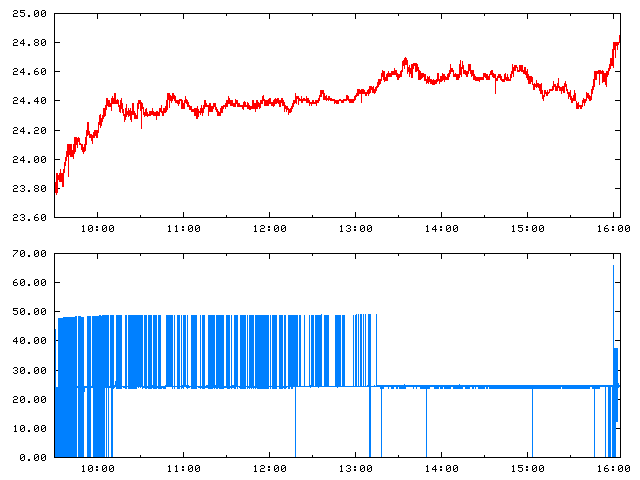
\includegraphics[width=0.7\linewidth]{gfx/m3l3_brownlees_fig1_trade_quote_oneday.png}
\par\smallskip{\small \textbf{Hình 1:} Dữ liệu giao dịch và báo giá của cổ phiếu General Electric vào ngày 11 tháng 11 năm 2002, từ 9:30:00 sáng đến 4:05:00 chiều. Chuỗi giá giao dịch theo từng tick (trên); chuỗi giá chào mua và chào bán theo từng tick (dưới).}
\end{figure}

Dữ liệu tần suất siêu cao (UHFD) thô vốn nổi tiếng là dễ chứa sai số, do đó cần áp dụng một phương pháp phát hiện và loại bỏ các giá trị sai số này trước khi tiến hành phân tích chuỗi thời gian. Thao tác xử lý dữ liệu sơ bộ này thường được gọi là lọc dữ liệu (filtering) hoặc làm sạch dữ liệu (data cleaning). Mục tiêu của nó là loại bỏ khỏi chuỗi thời gian tần suất siêu cao mọi quan sát không phản ánh đúng hoạt động thị trường thực tế; tuy nhiên trên thực tế, các phương pháp này dường như chỉ dừng ở mức phát hiện giá trị ngoại lai (outlier).

\begin{figure}[H]
\centering
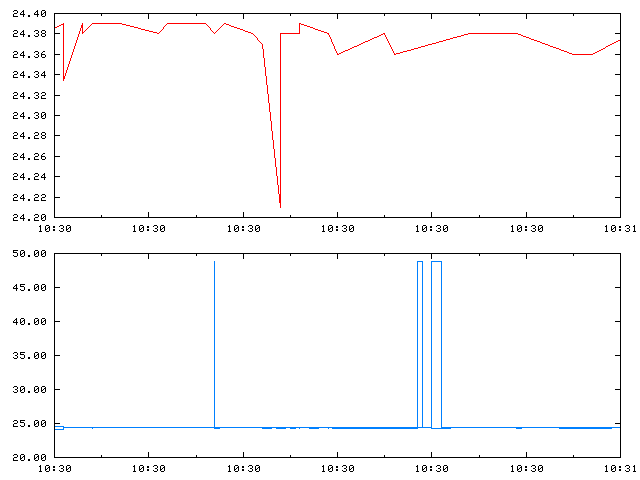
\includegraphics[width=0.7\linewidth]{gfx/m3l3_brownlees_fig2_trade_quote_oneminute.png}
\par\smallskip{\small \textbf{Hình 2:} Dữ liệu giao dịch và báo giá của cổ phiếu General Electric vào ngày 11 tháng 11 năm 2002, từ 10:30:00 sáng đến 10:31:00 sáng. Chuỗi giá giao dịch theo từng tick (trên); chuỗi giá chào mua và chào bán theo từng tick (dưới).}
\end{figure}

Nguồn gốc của các sai số này không thực sự rõ ràng. Falkenberry (2002) cho biết sai số xuất hiện cả trong các hệ thống giao dịch tự động hoàn toàn lẫn tự động một phần, chẳng hạn như Sàn Giao dịch Chứng khoán New York (NYSE). Theo tác giả này, cường độ giao dịch là yếu tố quyết định chính gây ra sai số: tốc độ giao dịch càng cao thì xác suất xảy ra sai sót khi báo cáo thông tin giao dịch càng lớn.

Phần lớn các quy trình làm sạch dữ liệu chỉ xử lý chuỗi giá theo từng giao dịch (tick-by-tick). Điều này có lẽ xuất phát từ việc tuy ``dễ dàng'' đánh giá một mức giá có phù hợp với điều kiện thị trường hiện tại hay không, nhưng lại khó hơn nhiều để đánh giá tính hợp lý của một khối lượng giao dịch nhất định. Do đó, đối với dữ liệu khối lượng, không có công thức làm sạch dữ liệu đặc thù nào ngoài việc đánh giá tính hợp lý của khối lượng dựa trên tính hợp lý của mức giá tương ứng, kết hợp với các phương pháp phát hiện giá trị ngoại lai thống kê cổ điển.

Hình 1 và Hình 2 lần lượt thể hiện dữ liệu giá giao dịch và báo giá của cổ phiếu General Electric trong một ngày và trong một phút. Có thể thấy dữ liệu giao dịch (trade) chính xác hơn nhiều so với dữ liệu báo giá (quote). Phù hợp với nhận định của Falkenberry (2002), một cách giải thích khả dĩ cho hiện tượng này là trong một ngày giao dịch, số lượng báo giá lớn hơn nhiều so với số lượng giao dịch thực hiện. Một cách giải thích khác là dữ liệu giao dịch ghi nhận các hợp đồng đã thực sự được khớp lệnh, chứ không chỉ là các đề nghị trao đổi đơn thuần, do đó các chủ thể thị trường thận trọng hơn nhiều khi báo cáo loại thông tin này so với báo giá. Một điểm đáng chú ý ở hai hình trên là chúng dường như cho thấy ít nhất một số sai số trong chuỗi dữ liệu là rất rõ ràng, dễ nhận thấy.

Trong các tài liệu đã có, một số thuật toán được đề xuất để loại bỏ các quan sát sai (xem Dacorogna et al. (2001) về thuật toán được Olsen \& Associates sử dụng để thực hiện công việc này trên dữ liệu tỷ giá hối đoái, vốn có vẻ phức tạp hơn nhiều so với mức cần thiết cho dữ liệu NYSE). Zhou (1996) đề cập một phương pháp đơn giản để kiểm định dữ liệu báo giá ngoại hối bằng cách so sánh mỗi báo giá với trung vị của ba quan sát liền trước và ba quan sát liền sau, rồi loại bỏ báo giá đó nếu nó nằm ngoài một khoảng cách cố định so với các trung vị này.

Thay vào đó, chúng tôi đề xuất một quy trình đã cho kết quả khả quan, như sẽ trình bày dưới đây. Gọi $\{p_i\}_{i=1}^{N}$ là một chuỗi giá theo từng giao dịch (tick-by-tick) đã được sắp xếp theo thứ tự. Quy trình mà chúng tôi đề xuất để loại bỏ giá trị ngoại lai là

\[
\big(\,|p_i - \bar{p}_i(k)| < 3\,s_i(k) + \gamma\,\big) =
\begin{cases}
\text{true} & \text{quan sát } i \text{ được giữ lại} \\
\text{false} & \text{quan sát } i \text{ bị loại bỏ}
\end{cases}
\]

trong đó $\bar p_i(k)$ và $s_i(k)$ lần lượt ký hiệu trung bình mẫu đã cắt tỉa 10\% (10\% trimmed mean) và độ lệch chuẩn mẫu của một vùng lân cận gồm $k$ quan sát xung quanh $i$, còn $\gamma$ là một \textit{tham số độ chi tiết} (granularity). Vùng lân cận các quan sát luôn được chọn sao cho một quan sát nhất định chỉ được so sánh với các quan sát thuộc cùng ngày giao dịch. Cụ thể, vùng lân cận của quan sát đầu tiên trong ngày là $k$ tick đầu tiên của ngày, vùng lân cận của quan sát cuối cùng trong ngày là $k$ tick cuối cùng của ngày, còn vùng lân cận của một giao dịch bất kỳ ở giữa ngày được tạo thành xấp xỉ bởi $k/2$ tick liền trước và $k/2$ tick liền sau, và tương tự như vậy cho các trường hợp khác. Ý tưởng đằng sau thuật toán này là đánh giá tính hợp lệ của một quan sát dựa trên khoảng cách tương đối của nó so với một vùng lân cận gồm các quan sát hợp lệ gần nhất. Vai trò của tham số $\gamma$ đặc biệt quan trọng. Các chuỗi dữ liệu tần suất siêu cao thường chứa các dãy giá bằng nhau liên tiếp, điều này khiến phương sai bằng 0; do đó, nên đưa vào một cận dưới dương cho các biến động giá luôn được xem là hợp lệ.

Cần lưu ý một số điểm quan trọng về việc lựa chọn các tham số của thuật toán, đó là $k$ và $\gamma$. Tham số $k$ nên được chọn dựa trên mức độ sôi động của giao dịch. Nếu giao dịch không quá sôi động, $k$ nên được chọn ``tương đối nhỏ'' để cửa sổ quan sát không chứa những mức giá quá xa nhau về thời gian. Ngược lại, nếu giao dịch rất sôi động, $k$ nên được chọn ``tương đối lớn'' để cửa sổ quan sát chứa đủ số lượng quan sát nhằm ước lượng chính xác các đặc điểm cục bộ của giá. Việc lựa chọn $\gamma$ nên là một bội số của mức biến động giá tối thiểu được phép đối với cổ phiếu cụ thể đang xét.

Quy trình này chắc chắn mang tính kinh nghiệm (heuristic), nhưng có ưu điểm là đơn giản và hiệu quả: chúng tôi sẽ cho thấy mức độ nhạy của một ví dụ minh họa trước cách chọn các tham số nói trên.

\section{3.2 Quản lý Dữ liệu}

Ngay cả khi UHFD đã được ``làm sạch'', việc xây dựng chuỗi thời gian phù hợp cho mục đích phân tích vẫn có thể khá phức tạp, bởi vì

\begin{itemize}
  \item dữ liệu có cấu trúc phức tạp, và
  \item không phải lúc nào cũng có một cách duy nhất và tối ưu để tổng hợp thông tin.
\end{itemize}

Trong các đoạn tiếp theo, chúng tôi sẽ trình bày một số đặc điểm riêng biệt xuất hiện trong dữ liệu cùng các phương pháp được đề xuất để xử lý chúng.

\noindent\textbf{Quan sát đồng thời.} Hình 3 trình bày 1 phút dữ liệu tần suất siêu cao gồm giá giao dịch, log-khối lượng giao dịch và hai chuỗi giá chào mua, giá chào bán. Lưu ý rằng mỗi dấu cộng trên đường giá giao dịch đánh dấu một giao dịch. Có thể thấy rằng có nhiều giao dịch được báo cáo tại cùng một thời điểm nhưng được khớp ở các mức giá khác nhau. Nhiều mức giá đồng thời khác nhau cũng xuất hiện trong dữ liệu báo giá.

\begin{figure}[H]
\centering
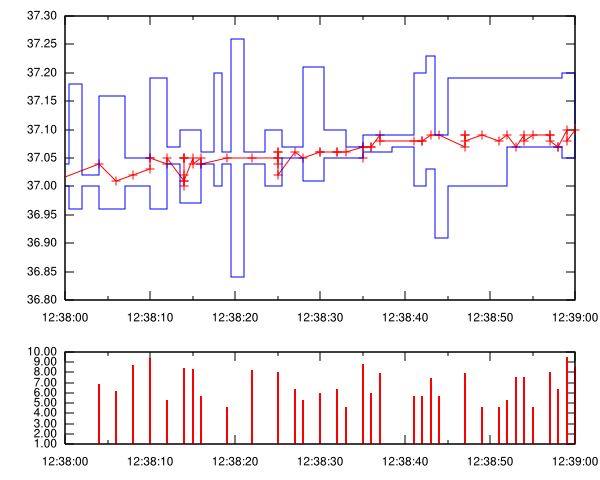
\includegraphics[width=0.7\linewidth]{gfx/m3l3_brownlees_fig3_trading_activity_minute.png}
\par\smallskip{\small \textbf{Hình 3:} Một phút hoạt động giao dịch của cổ phiếu General Electric vào ngày 21 tháng 3 năm 2002, từ 12:38 đến 12:39 chiều. Giá giao dịch nằm trong khoảng giá chào mua-chào bán (bảng trên). Mỗi dấu cộng trên đường giá giao dịch đánh dấu một giao dịch khác nhau. Log-khối lượng gắn với từng giao dịch (bảng dưới).}
\end{figure}

Có nhiều cách giải thích khác nhau cho hiện tượng này. Trước hết, cần lưu ý rằng các chứng khoán niêm yết trên NYSE cũng có thể được giao dịch trên các sàn khác, do đó việc có giao dịch và báo giá đồng thời ở các mức giá khác nhau là điều bình thường. Một cách giải thích khác cho hiện tượng này đối với dữ liệu giao dịch là việc khớp lệnh thị trường trên một sàn giao dịch đôi khi tạo ra nhiều hơn một báo cáo giao dịch. Cách giải thích thứ ba, cũng là cuối cùng, là ngay cả những giao dịch/báo giá không thực sự đồng thời cũng có thể bị ghi nhận là đồng thời do các sai số xấp xỉ khi báo cáo. Do đó, trên thực tế, rất thường gặp trường hợp có nhiều hơn một giao dịch và báo giá được báo cáo tại cùng một mốc thời gian.

Vì các mô hình tần suất siêu cao dùng để mô hình hóa dữ liệu tick-by-tick thường chỉ cần một quan sát cho mỗi mốc thời gian, nên cần thực hiện một hình thức tổng hợp (aggregation) nào đó. Đối với chuỗi giá tick-by-tick, thứ tự của các quan sát đồng thời được báo cáo dường như không mang nhiều ý nghĩa đặc biệt. Lấy giá trung vị có thể là một giải pháp hợp lý, xét đến bản chất rời rạc của dữ liệu tick-by-tick. Nếu sau đó còn tổng hợp thêm xuống các tần suất thấp hơn, việc chọn phương pháp tổng hợp càng ít quan trọng vì chênh lệch giữa các mức giá là không đáng kể, và các phương pháp đơn giản hơn như lấy giá cuối cùng hoặc giá đầu tiên của dãy quan sát cũng không nên gây ra vấn đề nào. Đối với khối lượng giao dịch hoặc số lượng giao dịch theo tick-by-tick, cách tổng hợp tự nhiên là thay thế các quan sát đồng thời bằng tổng khối lượng đồng thời và số lượng giao dịch đồng thời.

\noindent\textbf{Dữ liệu cách quãng không đều.} Đặc điểm nổi bật nhất của dữ liệu trình bày trong Hình 3 là các chuỗi thời gian được vẽ không đều đặn (irregular), nghĩa là khoảng thời gian phân cách hai quan sát liên tiếp là ngẫu nhiên. Thay vì làm việc trực tiếp với các quan sát tần suất siêu cao có khoảng cách thời gian không đều cho nhiều loại nghiên cứu khác nhau, người ta có thể muốn phân tích một chuỗi thời gian rời rạc với các khoảng thời gian cách đều nhau.

Gọi $\{(t_i,y_i)\}_{i=1}^{N}$ là một chuỗi thời gian không đều, trong đó $t_i$ và $y_i$ lần lượt biểu thị thời điểm và giá trị của quan sát thứ $i$, và gọi $\{(t_j^{*},y_j^{*})\}_{j=1}^{N^{*}}$ là chuỗi thời gian tần suất thấp hơn mà ta muốn xây dựng. Khi đó, vấn đề đặt ra là dùng một hàm tổng hợp phù hợp, tận dụng thông tin tần suất cao để thu được chuỗi quan sát $\{y_j^{*}\}_{j=1}^{N^{*}}$ của chuỗi đều. Vì ta đang tổng hợp thông tin tần suất cao xuống tần suất thấp hơn, dùng các hàm tổng hợp có dạng như sau có vẻ hợp lý:

\[
y_j^{*} = f\big(\{(t_i,y_i) \mid t_i \in (t_{j-1}^{*}, t_j^{*}]\}\big)
\]

điều này về cơ bản hàm ý rằng giá trị quan sát tổng hợp $y_j^{*}$ được xây dựng dựa trên toàn bộ thông tin sẵn có kể từ quan sát trước đó tại $t_{j-1}^{*}$ cho đến $t_j^{*}$.\footnote{Lưu ý rằng $f$ cũng có thể được định nghĩa thay thế như một hàm của $\{(t_i,y_i) \mid t_i \in [t_j^{*}, t_{j+1}^{*}), i=1,...,N\}$. Đây chỉ là vấn đề quy ước ký hiệu.}

Một số phương pháp đơn giản nhưng hữu ích, phù hợp với cách tiếp cận này, là:

\textbf{First:} $y_j^{*} = x_f$ trong đó $t_f = \min\{t_i \mid t_i \in (t_{j-1}^{*}, t_j^{*}]\}$

\textbf{Minimum:} $y_j^{*} = \min\{y_i \mid t_i \in (t_{j-1}^{*}, t_j^{*}]\}$

\textbf{Maximum:} $y_j^{*} = \max\{y_i \mid t_i \in (t_{j-1}^{*}, t_j^{*}]\}$

\textbf{Last:} $y_j^{*} = x_l$ trong đó $t_l = \max\{t_i \mid t_i \in (t_{j-1}^{*}, t_j^{*}]\}$

\textbf{Sum:} $y_j^{*} = \sum_{t_i \in (t_{j-1}^{*}, t_j^{*}]} y_i$

\textbf{Count:} $y_j^{*} = \#\{(y_i,t_i) \mid t_i \in (t_{j-1}^{*}, t_j^{*}]\}$

Trong bốn phương pháp đầu tiên, nếu tập $\{t_i \mid t_i \in [t_j^{*}, t_{j+1}^{*})\}$ rỗng thì quan sát thứ $j$ sẽ được coi là bị thiếu (missing). Các phương pháp ``First'', ``Minimum'', ``Maximum'' và ``Last'' có thể hữu ích khi xử lý chuỗi giá. Phương pháp ``Sum'' phù hợp để tổng hợp khối lượng, còn ``Count'' có thể được dùng để xác định số lượng giao dịch và báo giá.

Riêng đối với việc xây dựng chuỗi giá đều, Dacorogna et al. (2001) đề xuất một số phương pháp dựa trên việc nội suy tại $t_j^{*}$ từ quan sát liền trước và liền sau trong chuỗi:

\textbf{Previous Point Interpolation:} $y_j^{*} = y_p$ trong đó $t_p = \max\{t_i \mid t_i < t_j^{*}\}$

\textbf{Next Point Interpolation:} $y_j^{*} = y_n$ trong đó $t_n = \min\{t_i \mid t_i > t_j^{*}\}$

\textbf{Linear Point Interpolation:} $y_j^{*} = y_p + \dfrac{t_j^{*} - t_p}{t_n - t_p}(y_n - y_p)$

Tuy nhiên, vấn đề của các phương pháp này là chúng có thể dùng thông tin không thực sự có sẵn tại thời điểm $t_j^{*}$. Đối với các cổ phiếu thanh khoản cao, việc lựa chọn sơ đồ nội suy dường như không quá quan trọng vì vùng lân cận của $t^{*}$ sẽ chứa rất nhiều quan sát dày đặc, và các sơ đồ nội suy khác nhau sẽ cho kết quả xấp xỉ giống với phương pháp ``Last''. Ngược lại, kết quả có thể rất khác nhau đối với các cổ phiếu ít được giao dịch. Với các cổ phiếu này, chúng tôi cho rằng các sơ đồ nội suy không hoàn toàn thỏa đáng. Giả sử ta đang xây dựng một chuỗi giá tần suất cao có khoảng cách đều, chẳng hạn 5 phút. Điều thường xảy ra đối với các cổ phiếu ít được giao dịch và trong thời gian tạm ngừng giao dịch (halt) là sẽ có một số khoảng, chẳng hạn $(t_{j-1}^{*}, t_j^{*}]$, không chứa bất kỳ quan sát nào; do đó, trong trường hợp nội suy theo điểm liền trước, mức giá nội suy tại $t_j^{*}$ có thể thực chất là một mức giá thuộc về một thời điểm trước đó khá xa, chẳng hạn $(t_{j-k-1}^{*}, t_{j-k}^{*}]$ với $k>1$ nào đó.

Trong những trường hợp này, chúng tôi cho rằng thay vì gán một mức giá nội suy, sẽ hợp lý hơn nếu coi quan sát đó là bị thiếu. Nếu các chuỗi giá này được dùng để tạo lợi suất tần suất cao, cách làm này giúp tránh đưa vào chuỗi đã được điều chỉnh đều những dãy lợi suất bằng 0 kéo dài (nếu dùng nội suy theo điểm liền trước hoặc liền sau) hoặc những dãy lợi suất giống hệt nhau (nếu dùng nội suy tuyến tính), vốn sẽ làm tăng hiện tượng tự tương quan (serial correlation) và có khả năng gây ra vấn đề trong các thủ tục ước lượng phi tuyến bằng số.

\noindent\textbf{Hiện tượng nảy giá chào mua-chào bán (Bid-Ask Bounce).} Một hình mẫu thường gặp trong chuỗi giá giao dịch tick-by-tick là hiện tượng được gọi là \textit{nảy giá chào mua-chào bán} (bid-ask bounce), tức là xu hướng giá giao dịch dao động qua lại giữa giá chào mua và giá chào bán hiện hành. Roll (1984) đã cung cấp những hiểu biết sâu sắc về cơ chế này, vốn bắt nguồn từ vi cấu trúc thị trường (market microstructure).

Xét từ góc độ kinh tế, nguyên nhân của hiện tượng nảy giá chào mua-chào bán là do các giao dịch không nhất thiết luôn phát sinh từ sự xuất hiện của thông tin mới. Do đó, nếu không có sự kiện đáng kể nào xảy ra, các lệnh thị trường sẽ liên quan đến hoạt động mua và bán, và có xu hướng được khớp tại giá chào mua và giá chào bán hiện hành, tạo ra hình mẫu ``nảy giá'' nói trên.

Như có thể quan sát thấy trong Hình 3, giá giao dịch có xu hướng ``nảy'', nhưng hiện tượng này ít rõ rệt hơn nhiều so với các chuỗi dữ liệu khác, đặc biệt là so với các chuỗi dữ liệu NYSE thời kỳ đầu. Nguyên nhân là:

\begin{itemize}
  \item \textit{độ chi tiết} (granularity) giá khá mịn, tức là mức biến động giá tối thiểu trên NYSE kể từ tháng 1 năm 2000 là 0,01 USD;
  \item \textit{cải thiện giá} (price improvement), nghĩa là, khác với các sàn giao dịch khác, trên NYSE có thể thực hiện giao dịch với điều kiện tốt hơn so với báo giá hiện hành, do đó các lệnh thị trường mới sẽ không nhất thiết được khớp tại giá chào mua hoặc giá chào bán, làm giảm mức độ của hiện tượng ``nảy giá''.
\end{itemize}

Theo quan điểm truyền thống, hiện tượng nảy giá chào mua-chào bán có thể được coi là không chứa thông tin hữu ích, và có thể dẫn đến những vấn đề không mong muốn khi nó thể hiện các biến động giá vốn không thực sự xảy ra trên thực tế. Do đó, cần tìm cách loại bỏ hoặc giảm thiểu tác động của thành phần này lên dữ liệu. Có nhiều cách để đạt được mục tiêu này. Cách thứ nhất là không sử dụng chuỗi giá giao dịch để tính lợi suất mà thay vào đó sử dụng chuỗi giá trung bình báo giá (quote mid-price). Điều này khả thi trong bộ dữ liệu Trade and Quote (TAQ), nhưng lại gặp vấn đề về tính không đồng bộ giữa hai bộ dữ liệu. Ví dụ, dữ liệu báo giá lúc 3:00 chiều không thể so sánh trực tiếp với giá giao dịch được ghi nhận tại cùng thời điểm đó, và không thể thực sự dùng để loại bỏ vấn đề này trừ khi áp dụng quy tắc 5 giây (5-second rule) do Lee và Ready (1991) đề xuất. Gần đây, Vergote (2005) đã chỉ ra rằng độ trễ giữa báo giá và giao dịch thay đổi theo thời gian và theo từng cổ phiếu, đồng thời đề xuất một phiên bản mới của thuật toán do Lee và Ready (1991) đưa ra. Một giải pháp khác là xây dựng một thuật toán loại bỏ mọi biến động giá không vượt quá một ngưỡng nhất định (lớn hơn chênh lệch giá chào mua-chào bán) so với mức giá được chọn gần nhất.

\begin{figure}[H]
\centering
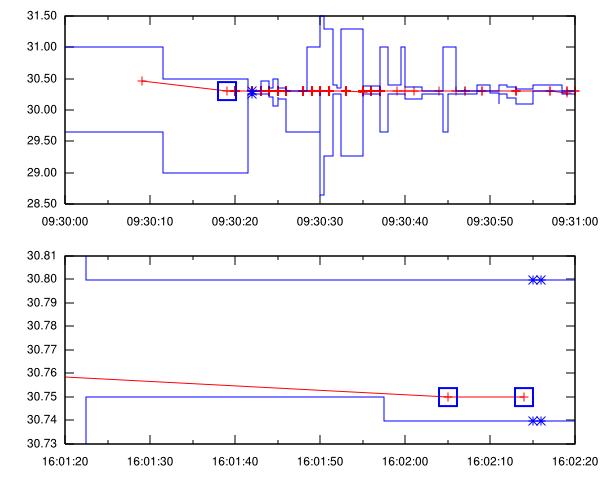
\includegraphics[width=0.7\linewidth]{gfx/m3l3_brownlees_fig4_open_close_minute.png}
\par\smallskip{\small \textbf{Hình 4:} Phút giao dịch đầu tiên và cuối cùng của cổ phiếu General Electric vào ngày 7 tháng 8 năm 2002. Mỗi dấu cộng trên đường giá giao dịch đánh dấu một giao dịch khác nhau. Các ô vuông trong bảng trên biểu thị giao dịch mở cửa của NYSE, còn các ô vuông trong bảng dưới biểu thị giao dịch đóng cửa của NYSE. Các dấu sao trên các đường giá chào mua-chào bán biểu thị báo giá mở cửa và đóng cửa của NYSE.}
\end{figure}

\noindent\textbf{Giá mở cửa và đóng cửa.} Một cách tự nhiên, người ta có thể kỳ vọng rằng giao dịch/báo giá đầu tiên (tương ứng, cuối cùng) trong ngày chính là giao dịch/báo giá mở cửa (tương ứng, đóng cửa) đã được ghi nhận chính thức. Tuy nhiên, từ Hình 4, thể hiện thời điểm đóng cửa và mở cửa của ngày giao dịch đang xét, có thể thấy rằng các giao dịch và báo giá đầu tiên trong ngày không phải là giao dịch và báo giá mở cửa chính thức của NYSE. Đáng chú ý là báo giá mở cửa cũng được ghi nhận sau giao dịch mở cửa. Vào thời điểm đóng cửa của NYSE trong cùng ngày đó, giao dịch cuối cùng được báo cáo trước 4:05 chiều thực sự là giao dịch đóng cửa, nhưng báo giá cuối cùng được báo cáo trong ngày lại không phải là báo giá đóng cửa. Do đó, việc xác định thời điểm mở cửa và đóng cửa của NYSE khó khăn hơn nhiều so với những gì người ta có thể nghĩ.

Ngày giao dịch chính thức của NYSE bắt đầu lúc 9:30 sáng và kết thúc lúc 4:00 chiều, nhưng trên thực tế, giao dịch sẽ bắt đầu muộn hơn một khoảng thời gian so với thời điểm mở cửa chính thức và tiếp tục kéo dài quá thời điểm đóng cửa, điều này hàm ý rằng thời điểm mở cửa và đóng cửa thực tế là ngẫu nhiên. Ngoài ra, rất thường gặp các báo cáo giao dịch và báo giá trong dữ liệu rõ ràng không thuộc về ngày giao dịch của NYSE, tức là các giao dịch trước 9:30 sáng và sau 4:00 chiều. Các bản ghi giao dịch và báo giá này có thể đến từ các sàn giao dịch khác hoặc từ các phiên giao dịch ngoài giờ (off-hours/crossing sessions) của NYSE, và do đó bị loại bỏ. Cuối cùng, để làm phức tạp thêm vấn đề, việc giao dịch thực tế của một cổ phiếu bắt đầu muộn hơn thời điểm mở cửa do độ trễ mở cửa (opening delays) không phải là điều hiếm gặp; ngoài ra, vào một số ngày đặc biệt (chẳng hạn những ngày trước kỳ nghỉ lễ), sàn giao dịch có thể đóng cửa sớm hơn.

Do đó, rất tiếc là không phải lúc nào cũng có thể xác định chính xác dữ liệu mở cửa và đóng cửa. Trường MODE trong dữ liệu báo giá (Bảng 1) cùng các trường G127 và COND trong dữ liệu giao dịch (Bảng 3) chứa một số cờ (flag) có thể dùng để xác định chính xác các giao dịch và báo giá mở cửa/đóng cửa, nhưng thông tin này không phải lúc nào cũng được báo cáo chính xác. Trên thực tế, giá giao dịch, giá chào mua hoặc giá chào bán đầu tiên và cuối cùng trong ngày không được kỳ vọng khác biệt đáng kể so với giá mở cửa và đóng cửa thực sự, và có thể được dùng làm biến đại diện (proxy). Tuy nhiên, điều này không đúng đối với khối lượng giao dịch và khối lượng báo giá.

Để nắm bắt đầy đủ mức giá đóng cửa trong ngày, chúng tôi áp dụng quy ước rằng khung giờ của ngày giao dịch trải dài từ 9:30 sáng đến 4:05 chiều. Quy ước này đảm bảo, ở mức độ lớn, rằng những mức giá đóng cửa được ghi nhận trễ cũng được tính đến. Khi sử dụng các khoảng thời gian cố định, chẳng hạn khi xây dựng chuỗi lợi suất 10 phút, khoảng thời gian cuối cùng trong ngày sẽ có độ dài danh nghĩa lớn hơn (trong ví dụ này là 15 phút, từ 3:50 chiều đến 4:05 chiều). Khi đó, lợi suất được tính bằng chênh lệch logarit (log-difference) giữa giá đóng cửa và mức giá ghi nhận lúc 3:50 chiều, coi là quan sát cuối cùng trong ngày.
